\documentclass[english]{article}
\usepackage[T1]{fontenc}
\usepackage[utf8]{inputenc}
\usepackage{csquotes, caption}
\usepackage[colorlinks=true, citecolor = blue]{hyperref}      % hyperlinks
\usepackage{multirow, amssymb, amsmath, graphicx, arydshln, url}
\usepackage[T1]{fontenc}
\usepackage{natbib}

\title{Supporting Information for ``Modelling publication bias and \textit{p}-hacking''\\ by Jonas Moss and Riccardo De Bin}

\author{}

\date{}

\begin{document}

\maketitle


\section*{Web Appendix A}

As mentioned in Section 2, any \textit{p}-hacking model can be written on the form of a selection model. Observe that
\begin{eqnarray*}
\int_{[0,1]}f_\alpha^{\star}(x_{i}\mid\theta_{i},\eta_{i}, u_i)d\omega(\alpha) & = & \int_{[0,1]}f(x_{i}\mid\theta_{i})P(u_i\in\left[0,\alpha\right]\mid\theta_{i},\eta_{i})^{-1}d\omega(\alpha)\\
 & = & f(x_{i}\mid\theta_{i})\int_{[0,u_i)}P(u_i\in\left[0,\alpha\right]\mid\theta_{i},\eta_{i})^{-1}d\omega(\alpha).
\end{eqnarray*}
where $f_\alpha^{\star}$ is the density $f^{\star}$ truncated so that the \textit{p}-value associated to $x_i$, $u_i$, lies in the interval $\left[0,\alpha\right)$. This is a publication bias model if $$h(u_i)=\int_{[0,u_i]}P(u_i\in\left[0,\alpha\right]\mid\theta_{i},\eta_{i})^{-1}d\omega(\alpha)$$ is bounded for each $u_i$ and $h(u_i)$ is independent of $\theta_{i},\eta_{i}$. While $h(u_i)$ can be bounded, it is typically dependent of $\theta_{i},\eta_{i}$, with the fixed effect model under complete selection for significance being a notable exception.

On the other hand, any selection model $f(x_{i};\theta_{i},\eta_{i})\rho(u_i)$ with $I =\int f(x;\theta_{i},\eta_{i})\rho(u_i)du_i<\infty$ can be written as a mixture model. For then there is a finite measure $d\omega(\alpha;\theta_{i},\eta_{i})$ satisfying 
\[
\rho(u_i)=\int_{[0,u_i)}\frac{1}{P(u_i\in\left[0,\alpha\right)\mid\theta,\eta)}d\omega(\alpha;\theta_{i},\eta_{i})
\]
Just take $d\omega(\alpha;\theta_{i},\eta_{i})=d\rho(\alpha)P(u_i\in\left[0,\alpha\right)\mid\theta_{i},\eta_{i})$, where $d\rho(\alpha)$ is defined by $\int_{0}^{u_i}d\rho(\alpha)=\rho(u_i)$. The size of the measure is
\begin{eqnarray*}
\int_{0}^{1}d\omega(\alpha;\theta_{i},\eta_{i}) & = & \int_{0}^{1}P(u_i\in\left[0,\alpha\right)\mid\theta_{i},\eta_{i})d\rho(\alpha)\\
 & = & \int_{0}^{1}f(u_i;\theta_{i},\eta_{i})\int_{0}^{u_i}d\rho(\alpha)du_i\\
 & = & I
\end{eqnarray*}
Hence $I_{\theta,\eta}d\omega'(\alpha;\theta_{i},\eta_{i})$ is a probability measure. This probability measure makes 
\[
I^{-1}f(x_{i};\theta_{i},\eta_{i})\rho(u_i)=\int_{[0,1]}f_\alpha(x_{i};\theta_{i},\eta_{i})d\omega'(\alpha)
\]
as can be seen by the following computation,
\begin{eqnarray*}
I^{-1}f(x_{i};\theta_{i},\eta_{i})\rho(u_i) & = & I^{-1}\int_{[0,u_i)}\frac{f(x_{i};\theta_{i},\eta_{i})}{P(u_i\in\left[0,\alpha\right)\mid\theta_{i},\eta_{i})}d\omega(\alpha)\\
 & = & I^{-1}\int_{[0,1]}\frac{f(x_{i};\theta,\eta)1_{\left[0,\alpha\right)}(u_i)}{P(u_i\in\left[0,\alpha\right)\mid\theta_{i},\eta_{i})}d\omega(\alpha)\\
 & = & I^{-1}\int_{[0,1]}f_\alpha(x_{i};\theta_{i},\eta_{i})d\omega(\alpha)\\
 & = & \int_{[0,1]}f_\alpha(x;\theta_{i},\eta_{i})d\omega'(\alpha)
\end{eqnarray*}

Proposition 1 shows the form of the one-sided normal step function selection probability publication bias model when it is written as a mixture model of the form (5). But most such mixture models are not true \textit{p}-hacking models, as the mixing probabilities $\pi_{i}^{\star}$ depend on $\theta$. There is no way for the \textit{p}-hacker to know
$\theta$, so we cannot regard the publication bias model as a \textit{p}-hacking model.

\newpage

\section*{Web Appendix B}

%\subsection*{Inverse Gamma prior on $\tau^2$}

\begin{table}[ht]
\centering
\caption*{\noindent Table C.1: {\bf Inverse Gamma prior, no publication bias, no 
                    \textit{p}-hacking.} Posterior means and 
                    standard deviations from the \textit{p}-hacking and 
                    publication bias models when the data are simulated 
                    from the normal random effects meta-analysis model.}
\label{tab:Simulation_ph}
\begin{tabular}{lllrrrrrr}
   \multicolumn{3}{r}{\textbf{True values}} & 
       \multicolumn{2}{c}{\textbf{\textit{p}-hacking model}} &
       \multicolumn{2}{c}{\textbf{Public. bias model}} &
       \multicolumn{2}{c}{\textbf{Classical model}}\\$\tau$ & $\theta_0$ & $n$ & \multicolumn{1}{c}{$\widehat{\theta_0}$} & \multicolumn{1}{c}{$\widehat{\tau}$} & \multicolumn{1}{c}{$\widehat{\theta_0}$} & \multicolumn{1}{c}{$\widehat{\tau}$} & \multicolumn{1}{c}{$\widehat{\theta_0}$} & \multicolumn{1}{c}{$\widehat{\tau}$} \\ 
   \hline
  \multirow{9}{*}{$0.1$} & \multirow{3}{*}{$0$} & 5 & -0.03 (0.08) & 0.18 (0.08) & -0.06 (0.06) & 0.14 (0.07) & 0.00 (0.07) & 0.20 (0.09) \\ 
  & & 30 & -0.02 (0.03) & 0.08 (0.03) & -0.02 (0.03) & 0.07 (0.03) & 0.00 (0.03) & 0.10 (0.04) \\ 
  & & 100 & -0.01 (0.02) & 0.08 (0.02) & -0.02 (0.02) & 0.07 (0.02) & 0.00 (0.02) & 0.09 (0.02) \\ 
   \cdashline{3-9}
 & \multirow{3}{*}{$0.2$} & 5 & 0.12 (0.08) & 0.20 (0.07) & 0.08 (0.06) & 0.15 (0.06) & 0.19 (0.08) & 0.18 (0.07) \\ 
  & & 30 & 0.17 (0.04) & 0.09 (0.04) & 0.15 (0.03) & 0.08 (0.04) & 0.20 (0.03) & 0.09 (0.03) \\ 
  & & 100 & 0.18 (0.02) & 0.09 (0.03) & 0.17 (0.02) & 0.09 (0.03) & 0.20 (0.02) & 0.09 (0.02) \\ 
   \cdashline{3-9}
 & \multirow{3}{*}{$0.8$} & 5 & 0.78 (0.07) & 0.20 (0.10) & 0.64 (0.13) & 0.32 (0.14) & 0.79 (0.07) & 0.18 (0.08) \\ 
  & & 30 & 0.80 (0.04) & 0.10 (0.04) & 0.79 (0.04) & 0.10 (0.04) & 0.80 (0.03) & 0.10 (0.04) \\ 
  & & 100 & 0.80 (0.02) & 0.09 (0.03) & 0.80 (0.02) & 0.09 (0.03) & 0.80 (0.02) & 0.09 (0.03) \\ 
  \cline{2-9}
\multirow{9}{*}{$0.5$} & \multirow{3}{*}{$0$} & 5 & -0.08 (0.20) & 0.56 (0.22) & -0.24 (0.18) & 0.50 (0.21) & -0.03 (0.21) & 0.58 (0.21) \\ 
  & & 30 & -0.03 (0.08) & 0.50 (0.07) & -0.14 (0.08) & 0.46 (0.07) & 0.00 (0.08) & 0.50 (0.07) \\ 
  & & 100 & -0.02 (0.05) & 0.50 (0.04) & -0.08 (0.06) & 0.48 (0.04) & 0.00 (0.05) & 0.50 (0.04) \\ 
   \cdashline{3-9}
 & \multirow{3}{*}{$0.2$} & 5 & 0.16 (0.24) & 0.60 (0.19) & -0.04 (0.20) & 0.58 (0.2) & 0.20 (0.24) & 0.60 (0.19) \\ 
  & & 30 & 0.16 (0.08) & 0.52 (0.07) & 0.03 (0.09) & 0.50 (0.07) & 0.19 (0.08) & 0.52 (0.07) \\ 
  & & 100 & 0.18 (0.06) & 0.51 (0.04) & 0.10 (0.06) & 0.50 (0.04) & 0.20 (0.06) & 0.50 (0.04) \\ 
   \cdashline{3-9}
 & \multirow{3}{*}{$0.8$} & 5 & 0.73 (0.26) & 0.61 (0.17) & 0.40 (0.28) & 0.74 (0.18) & 0.75 (0.25) & 0.58 (0.17) \\ 
  & & 30 & 0.77 (0.09) & 0.53 (0.07) & 0.60 (0.12) & 0.60 (0.09) & 0.79 (0.08) & 0.51 (0.07) \\ 
  & & 100 & 0.80 (0.06) & 0.52 (0.04) & 0.71 (0.07) & 0.55 (0.04) & 0.81 (0.05) & 0.51 (0.04) \\ 
  \hline
\end{tabular}
\end{table}



\begin{table}[ht]
\centering
\caption*{\noindent Table C.2: {\bf Inverse Gamma prior, publication bias.} 
                    Posterior means and standard deviations from the 
                    \textit{p}-hacking, publication bias, and uncorrected models 
                    when the data are simulated from the publication 
                    bias model with cutoffs at $0.025$ and $0.05$, 
                    with selection probabilities equal to $1$, $0.7$, 
                    and $0.1$ in the intervals $[0, 0.025)$, $[0.025, 0.05)$, 
                    and $[0.5, 1]$.} 
\label{tab:Simulation_pb}
\begin{tabular}{lllrrrrrr}
   \multicolumn{3}{r}{\textbf{True values}} & 
       \multicolumn{2}{c}{\textbf{\textit{p}-hacking model}} &
       \multicolumn{2}{c}{\textbf{Public.\ bias model}} &
       \multicolumn{2}{c}{\textbf{Uncorrected model}}\\$\tau$ & $\theta_0$ & $n$ & \multicolumn{1}{c}{$\widehat{\theta_0}$} & \multicolumn{1}{c}{$\widehat{\tau}$} & \multicolumn{1}{c}{$\widehat{\theta_0}$} & \multicolumn{1}{c}{$\widehat{\tau}$} & \multicolumn{1}{c}{$\widehat{\theta_0}$} & \multicolumn{1}{c}{$\widehat{\tau}$} \\ 
   \hline
  \multirow{9}{*}{$0.1$} & \multirow{3}{*}{$0$} & 5 & -0.02 (0.11) & 0.21 (0.08) & 0.00 (0.08) & 0.16 (0.07) & 0.12 (0.08) & 0.22 (0.10) \\ 
  & & 30 & 0.03 (0.05) & 0.12 (0.04) & 0.02 (0.04) & 0.10 (0.03) & 0.14 (0.04) & 0.15 (0.04) \\ 
  & & 100 & 0.02 (0.02) & 0.11 (0.03) & 0.01 (0.02) & 0.09 (0.02) & 0.13 (0.02) & 0.16 (0.02) \\
   \cdashline{3-9}
 & \multirow{3}{*}{$0.2$} & 5 & 0.12 (0.13) & 0.29 (0.10) & 0.10 (0.07) & 0.21 (0.09) & 0.33 (0.06) & 0.16 (0.07) \\ 
  & & 30 & 0.22 (0.05) & 0.12 (0.05) & 0.19 (0.05) & 0.10 (0.04) & 0.33 (0.03) & 0.06 (0.03) \\ 
  & & 100 & 0.23 (0.03) & 0.11 (0.03) & 0.19 (0.05) & 0.09 (0.03) & 0.33 (0.02) & 0.04 (0.02) \\
   \cdashline{3-9}
 & \multirow{3}{*}{$0.8$} & 5 & 0.79 (0.11) & 0.21 (0.10) & 0.65 (0.17) & 0.31 (0.13) & 0.80 (0.10) & 0.19 (0.07) \\ 
  & & 30 & 0.80 (0.03) & 0.10 (0.04) & 0.80 (0.03) & 0.10 (0.05) & 0.80 (0.03) & 0.10 (0.04) \\ 
  & & 100 & 0.80 (0.02) & 0.09 (0.03) & 0.80 (0.02) & 0.10 (0.03) & 0.80 (0.02) & 0.09 (0.03) \\ 
  \cline{2-9}
\multirow{9}{*}{$0.5$} & \multirow{3}{*}{$0$} & 5 & 0.30 (0.26) & 0.53 (0.20) & 0.03 (0.22) & 0.55 (0.19) & 0.40 (0.22) & 0.48 (0.20) \\ 
  & & 30 & 0.34 (0.10) & 0.47 (0.08) & 0.00 (0.17) & 0.49 (0.08) & 0.42 (0.09) & 0.42 (0.09) \\ 
  & & 100 & 0.35 (0.05) & 0.46 (0.04) & 0.00 (0.10) & 0.49 (0.05) & 0.43 (0.04) & 0.42 (0.04) \\ 
   \cdashline{3-9}
 & \multirow{3}{*}{$0.2$} & 5 & 0.48 (0.22) & 0.55 (0.19) & 0.17 (0.22) & 0.61 (0.19) & 0.55 (0.19) & 0.47 (0.21) \\ 
  & & 30 & 0.52 (0.09) & 0.43 (0.08) & 0.18 (0.16) & 0.51 (0.09) & 0.57 (0.08) & 0.37 (0.08) \\ 
  & & 100 & 0.50 (0.05) & 0.43 (0.05) & 0.20 (0.13) & 0.50 (0.05) & 0.56 (0.04) & 0.38 (0.04) \\ 
   \cdashline{3-9}
 & \multirow{3}{*}{$0.8$} & 5 & 0.81 (0.22) & 0.52 (0.20) & 0.48 (0.27) & 0.68 (0.21) & 0.85 (0.20) & 0.47 (0.18) \\ 
  & & 30 & 0.91 (0.09) & 0.45 (0.07) & 0.69 (0.18) & 0.57 (0.11) & 0.93 (0.08) & 0.42 (0.07) \\ 
  & & 100 & 0.91 (0.05) & 0.44 (0.04) & 0.75 (0.13) & 0.53 (0.08) & 0.93 (0.05) & 0.41 (0.04) \\ \hline
\end{tabular}
\end{table}

\begin{table}[ht]
\centering
\caption*{\noindent Table C.3: {\bf  Inverse Gamma prior, \textit{p}-hacking.} Posterior means and 
                    standard deviations from the \textit{p}-hacking, 
                    publication bias, and uncorrected models when the data are simulated 
                    from the \textit{p}-hacking model with cutoffs at
                    $0.025$ and $0.05$, with \textit{p}-hacking probabilities
                    equal to $0.6$, $0.3$, and $0.1$ for $\alpha = 0.025, 0.05$, and $1$} 
\label{tab:Simulation_ph}
\begin{tabular}{lllrrrrrr}
   \multicolumn{3}{r}{\textbf{True values}} & 
       \multicolumn{2}{c}{\textbf{\textit{p}-hacking model}} &
       \multicolumn{2}{c}{\textbf{Public. bias model}} &
       \multicolumn{2}{c}{\textbf{Uncorrected model}}\\$\tau$ & $\theta_0$ & $n$ & \multicolumn{1}{c}{$\widehat{\theta_0}$} & \multicolumn{1}{c}{$\widehat{\tau}$} & \multicolumn{1}{c}{$\widehat{\theta_0}$} & \multicolumn{1}{c}{$\widehat{\tau}$} & \multicolumn{1}{c}{$\widehat{\theta_0}$} & \multicolumn{1}{c}{$\widehat{\tau}$} \\ 
   \hline
  \multirow{9}{*}{$0.1$} & \multirow{3}{*}{$0$} & 5 & -0.06 (0.13) & 0.28 (0.07) & 0.04 (0.07) & 0.17 (0.05) & 0.29 (0.07) & 0.15 (0.08) \\ 
  & & 30 & -0.02 (0.07) & 0.13 (0.04) & 0.02 (0.06) & 0.06 (0.02) & 0.28 (0.02) & 0.06 (0.03) \\ 
  & & 100 & -0.01 (0.04) & 0.10 (0.04) & -0.01 (0.05) & 0.05 (0.03) & 0.29 (0.01) & 0.03 (0.02) \\ 
   \cdashline{3-9}
 & \multirow{3}{*}{$0.2$} & 5 & 0.13 (0.15) & 0.29 (0.09) & 0.09 (0.07) & 0.22 (0.08) & 0.35 (0.06) & 0.14 (0.06) \\ 
  & & 30 & 0.18 (0.06) & 0.11 (0.04) & 0.15 (0.05) & 0.09 (0.03) & 0.34 (0.02) & 0.04 (0.01) \\ 
  & & 100 & 0.20 (0.03) & 0.09 (0.04) & 0.16 (0.04) & 0.08 (0.03) & 0.34 (0.01) & 0.02 (0.01) \\ 
   \cdashline{3-9}
 & \multirow{3}{*}{$0.8$} & 5 & 0.78 (0.08) & 0.20 (0.08) & 0.63 (0.14) & 0.32 (0.12) & 0.78 (0.08) & 0.19 (0.07) \\ 
  & & 30 & 0.79 (0.04) & 0.10 (0.04) & 0.79 (0.04) & 0.10 (0.04) & 0.79 (0.03) & 0.10 (0.04) \\ 
  & & 100 & 0.80 (0.02) & 0.10 (0.02) & 0.80 (0.02) & 0.10 (0.03) & 0.80 (0.02) & 0.09 (0.02) \\ 
  \cline{2-9}
\multirow{9}{*}{$0.5$} & \multirow{3}{*}{$0$} & 5 & 0.06 (0.20) & 0.47 (0.19) & 0.02 (0.10) & 0.35 (0.21) & 0.37 (0.12) & 0.27 (0.18) \\ 
  & & 30 & 0.07 (0.09) & 0.44 (0.09) & -0.25 (0.19) & 0.36 (0.11) & 0.37 (0.05) & 0.24 (0.10) \\ 
  & & 100 & 0.06 (0.06) & 0.44 (0.04) & -0.36 (0.15) & 0.37 (0.06) & 0.36 (0.03) & 0.25 (0.05) \\ 
   \cdashline{3-9}
 & \multirow{3}{*}{$0.2$} & 5 & 0.24 (0.21) & 0.52 (0.20) & 0.05 (0.12) & 0.47 (0.21) & 0.45 (0.13) & 0.33 (0.18) \\ 
  & & 30 & 0.24 (0.10) & 0.47 (0.08) & -0.20 (0.20) & 0.46 (0.11) & 0.45 (0.06) & 0.29 (0.08) \\ 
  & & 100 & 0.23 (0.06) & 0.47 (0.04) & -0.30 (0.15) & 0.48 (0.06) & 0.46 (0.04) & 0.28 (0.04) \\
   \cdashline{3-9}
 & \multirow{3}{*}{$0.8$} & 5 & 0.69 (0.18) & 0.60 (0.20) & 0.31 (0.19) & 0.74 (0.19) & 0.76 (0.14) & 0.51 (0.18) \\ 
  & & 30 & 0.80 (0.10) & 0.51 (0.08) & 0.39 (0.25) & 0.66 (0.12) & 0.85 (0.08) & 0.44 (0.07) \\ 
  & & 100 & 0.81 (0.05) & 0.50 (0.04) & 0.43 (0.19) & 0.65 (0.09) & 0.86 (0.04) & 0.43 (0.03) \\ 
  \hline
\end{tabular}
\end{table}

\newpage

%\subsection*{Uniform prior on $\tau$}


\begin{table}[ht]
\centering
\caption*{\noindent Table C.4: {\bf Uniform prior, no publication bias, no 
                    \textit{p}-hacking.} Posterior means and 
                    standard deviations from the \textit{p}-hacking and 
                    publication bias models when the data are simulated 
                    from the normal random effects meta-analysis model.}
\label{tab:Simulation_ph}
\begin{tabular}{lllrrrrrr}
   \multicolumn{3}{r}{\textbf{True values}} & 
       \multicolumn{2}{c}{\textbf{\textit{p}-hacking model}} &
       \multicolumn{2}{c}{\textbf{Public. bias model}} &
       \multicolumn{2}{c}{\textbf{Classical model}}\\$\tau$ & $\theta_0$ & $n$ & \multicolumn{1}{c}{$\widehat{\theta_0}$} & \multicolumn{1}{c}{$\widehat{\tau}$} & \multicolumn{1}{c}{$\widehat{\theta_0}$} & \multicolumn{1}{c}{$\widehat{\tau}$} & \multicolumn{1}{c}{$\widehat{\theta_0}$} & \multicolumn{1}{c}{$\widehat{\tau}$} \\ 
   \hline
  \multirow{9}{*}{$0.1$} & \multirow{3}{*}{$0$} & 5 & -0.03 (0.07) & 0.17 (0.06) & -0.06 (0.07) & 0.12 (0.05) & -0.01 (0.08) & 0.18 (0.07) \\ 
  & & 30 & -0.02 (0.03) & 0.08 (0.03) & -0.02 (0.03) & 0.07 (0.03) & 0.00 (0.04) & 0.10 (0.03) \\ 
  & & 100 & -0.01 (0.02) & 0.08 (0.03) & -0.02 (0.02) & 0.07 (0.03) & 0.00 (0.02) & 0.10 (0.03) \\ 
   \cdashline{3-9}
 & \multirow{3}{*}{$0.2$} & 5 & 0.12 (0.09) & 0.21 (0.09) & 0.09 (0.07) & 0.16 (0.08) & 0.19 (0.08) & 0.18 (0.08) \\ 
  & & 30 & 0.17 (0.03) & 0.09 (0.04) & 0.15 (0.03) & 0.09 (0.03) & 0.20 (0.03) & 0.10 (0.03) \\ 
  & & 100 & 0.18 (0.02) & 0.09 (0.03) & 0.17 (0.02) & 0.09 (0.03) & 0.20 (0.02) & 0.09 (0.02) \\ 
   \cdashline{3-9}
 & \multirow{3}{*}{$0.8$} & 5 & 0.77 (0.09) & 0.20 (0.08) & 0.62 (0.14) & 0.31 (0.13) & 0.77 (0.08) & 0.18 (0.07) \\ 
  & & 30 & 0.80 (0.04) & 0.10 (0.04) & 0.80 (0.04) & 0.10 (0.04) & 0.80 (0.03) & 0.10 (0.04) \\ 
  & & 100 & 0.80 (0.02) & 0.10 (0.02) & 0.80 (0.02) & 0.10 (0.03) & 0.80 (0.02) & 0.10 (0.02) \\ 
  \cline{2-9}
\multirow{9}{*}{$0.5$} & \multirow{3}{*}{$0$} & 5 & -0.03 (0.20) & 0.55 (0.19) & -0.21 (0.17) & 0.49 (0.19) & 0.01 (0.20) & 0.57 (0.19) \\ 
  & & 30 & -0.02 (0.10) & 0.51 (0.08) & -0.13 (0.10) & 0.48 (0.08) & 0.00 (0.10) & 0.51 (0.08) \\ 
  & & 100 & -0.02 (0.05) & 0.50 (0.04) & -0.08 (0.05) & 0.48 (0.04) & 0.00 (0.05) & 0.50 (0.04) \\ 
   \cdashline{3-9}
 & \multirow{3}{*}{$0.2$} & 5 & 0.20 (0.22) & 0.57 (0.19) & -0.02 (0.17) & 0.57 (0.19) & 0.24 (0.21) & 0.57 (0.18) \\ 
  & & 30 & 0.17 (0.10) & 0.52 (0.08) & 0.05 (0.10) & 0.50 (0.08) & 0.20 (0.10) & 0.51 (0.08) \\ 
  & & 100 & 0.19 (0.06) & 0.51 (0.04) & 0.11 (0.06) & 0.50 (0.04) & 0.20 (0.06) & 0.50 (0.04) \\ 
   \cdashline{3-9}
 & \multirow{3}{*}{$0.8$} & 5 & 0.74 (0.23) & 0.61 (0.23) & 0.41 (0.24) & 0.75 (0.23) & 0.77 (0.22) & 0.58 (0.22) \\ 
  & & 30 & 0.79 (0.10) & 0.53 (0.07) & 0.60 (0.14) & 0.61 (0.08) & 0.81 (0.10) & 0.51 (0.07) \\ 
  & & 100 & 0.78 (0.06) & 0.52 (0.04) & 0.70 (0.07) & 0.55 (0.04) & 0.80 (0.06) & 0.51 (0.04) \\ 
  \hline
\end{tabular}
\end{table}



\begin{table}[ht]
\centering
\caption*{\noindent Table C.5: {\bf Uniform prior, publication bias.} 
                    Posterior means and standard deviations from the 
                    \textit{p}-hacking, publication bias, and uncorrected models 
                    when the data are simulated from the publication 
                    bias model with cutoffs at $0.025$ and $0.05$, 
                    with selection probabilities equal to $1$, $0.7$, 
                    and $0.1$ in the intervals $[0, 0.025)$, $[0.025, 0.05)$, 
                    and $[0.5, 1]$.} 
\label{tab:Simulation_pb}
\begin{tabular}{lllrrrrrr}
   \multicolumn{3}{r}{\textbf{True values}} & 
       \multicolumn{2}{c}{\textbf{\textit{p}-hacking model}} &
       \multicolumn{2}{c}{\textbf{Public.\ bias model}} &
       \multicolumn{2}{c}{\textbf{Uncorrected model}}\\$\tau$ & $\theta_0$ & $n$ & \multicolumn{1}{c}{$\widehat{\theta_0}$} & \multicolumn{1}{c}{$\widehat{\tau}$} & \multicolumn{1}{c}{$\widehat{\theta_0}$} & \multicolumn{1}{c}{$\widehat{\tau}$} & \multicolumn{1}{c}{$\widehat{\theta_0}$} & \multicolumn{1}{c}{$\widehat{\tau}$} \\ 
   \hline
  \multirow{9}{*}{$0.1$} & \multirow{3}{*}{$0$} & 5 & -0.01 (0.11) & 0.24 (0.09) & -0.01 (0.08) & 0.18 (0.08) & 0.13 (0.09) & 0.24 (0.10) \\ 
  & & 30 & 0.02 (0.05) & 0.12 (0.04) & 0.01 (0.04) & 0.10 (0.03) & 0.13 (0.04) & 0.16 (0.04) \\ 
  & & 100 & 0.03 (0.03) & 0.12 (0.03) & 0.01 (0.02) & 0.10 (0.02) & 0.14 (0.02) & 0.16 (0.02) \\ 
   \cdashline{3-9}
 & \multirow{3}{*}{$0.2$} & 5 & 0.16 (0.13) & 0.27 (0.08) & 0.12 (0.06) & 0.21 (0.06) & 0.33 (0.06) & 0.15 (0.06) \\ 
  & & 30 & 0.23 (0.05) & 0.12 (0.05) & 0.19 (0.06) & 0.10 (0.04) & 0.33 (0.03) & 0.06 (0.02) \\ 
  & & 100 & 0.24 (0.03) & 0.10 (0.03) & 0.20 (0.04) & 0.10 (0.03) & 0.33 (0.02) & 0.04 (0.02) \\ 
   \cdashline{3-9}
 & \multirow{3}{*}{$0.8$} & 5 & 0.80 (0.07) & 0.19 (0.08) & 0.66 (0.13) & 0.31 (0.13) & 0.80 (0.07) & 0.18 (0.07) \\ 
  & & 30 & 0.80 (0.03) & 0.10 (0.04) & 0.79 (0.04) & 0.11 (0.04) & 0.80 (0.03) & 0.10 (0.04) \\ 
  & & 100 & 0.80 (0.02) & 0.09 (0.03) & 0.80 (0.02) & 0.09 (0.02) & 0.80 (0.02) & 0.09 (0.02) \\ 
  \cline{2-9}
\multirow{9}{*}{$0.5$} & \multirow{3}{*}{$0$} & 5 & 0.36 (0.24) & 0.54 (0.20) & 0.07 (0.23) & 0.57 (0.18) & 0.45 (0.21) & 0.47 (0.22) \\ 
  & & 30 & 0.39 (0.10) & 0.47 (0.08) & 0.04 (0.17) & 0.51 (0.08) & 0.45 (0.08) & 0.42 (0.08) \\ 
  & & 100 & 0.36 (0.06) & 0.48 (0.04) & 0.00 (0.12) & 0.51 (0.05) & 0.43 (0.05) & 0.43 (0.05) \\ 
   \cdashline{3-9}
 & \multirow{3}{*}{$0.2$} & 5 & 0.41 (0.22) & 0.53 (0.18) & 0.11 (0.20) & 0.58 (0.18) & 0.49 (0.17) & 0.46 (0.20) \\ 
  & & 30 & 0.50 (0.08) & 0.45 (0.08) & 0.15 (0.18) & 0.52 (0.09) & 0.55 (0.07) & 0.39 (0.08) \\ 
  & & 100 & 0.51 (0.05) & 0.43 (0.05) & 0.17 (0.13) & 0.51 (0.06) & 0.56 (0.04) & 0.38 (0.05) \\
  \cdashline{3-9}
 & \multirow{3}{*}{$0.8$} & 5 & 0.86 (0.16) & 0.52 (0.19) & 0.51 (0.23) & 0.70 (0.20) & 0.89 (0.15) & 0.49 (0.17) \\ 
  & & 30 & 0.90 (0.09) & 0.46 (0.07) & 0.67 (0.19) & 0.58 (0.11) & 0.92 (0.08) & 0.43 (0.06) \\ 
  & & 100 & 0.91 (0.05) & 0.44 (0.04) & 0.76 (0.11) & 0.52 (0.07) & 0.93 (0.04) & 0.41 (0.03) \\ \hline
\end{tabular}
\end{table}

\begin{table}[ht]
\centering
\caption*{\noindent Table C.6: {\bf Uniform prior, \textit{p}-hacking.} Posterior means and 
                    standard deviations from the \textit{p}-hacking, 
                    publication bias, and uncorrected models when the data are simulated 
                    from the \textit{p}-hacking model with cutoffs at
                    $0.025$ and $0.05$, with \textit{p}-hacking probabilities
                    equal to $0.6$, $0.3$, and $0.1$ for $\alpha = 0.025, 0.05$, and $1$} 
\label{tab:Simulation_ph}
\begin{tabular}{lllrrrrrr}
   \multicolumn{3}{r}{\textbf{True values}} & 
       \multicolumn{2}{c}{\textbf{\textit{p}-hacking model}} &
       \multicolumn{2}{c}{\textbf{Public. bias model}} &
       \multicolumn{2}{c}{\textbf{Uncorrected model}}\\$\tau$ & $\theta_0$ & $n$ & \multicolumn{1}{c}{$\widehat{\theta_0}$} & \multicolumn{1}{c}{$\widehat{\tau}$} & \multicolumn{1}{c}{$\widehat{\theta_0}$} & \multicolumn{1}{c}{$\widehat{\tau}$} & \multicolumn{1}{c}{$\widehat{\theta_0}$} & \multicolumn{1}{c}{$\widehat{\tau}$} \\ 
   \hline
  \multirow{9}{*}{$0.1$} & \multirow{3}{*}{$0$} & 5 & -0.07 (0.14) & 0.28 (0.08) & 0.04 (0.07) & 0.17 (0.07) & 0.29 (0.06) & 0.15 (0.09) \\ 
  & & 30 & -0.02 (0.08) & 0.13 (0.05) & 0.00 (0.07) & 0.07 (0.03) & 0.29 (0.03) & 0.05 (0.04) \\ 
  & & 100 & -0.01 (0.04) & 0.11 (0.04) & -0.02 (0.05) & 0.06 (0.02) & 0.28 (0.01) & 0.03 (0.02) \\ 
   \cdashline{3-9}
 & \multirow{3}{*}{$0.2$} & 5 & 0.11 (0.13) & 0.28 (0.09) & 0.09 (0.05) & 0.20 (0.05) & 0.34 (0.05) & 0.13 (0.05) \\ 
  & & 30 & 0.20 (0.05) & 0.11 (0.05) & 0.16 (0.06) & 0.09 (0.04) & 0.34 (0.02) & 0.04 (0.02) \\ 
  & & 100 & 0.20 (0.03) & 0.09 (0.03) & 0.17 (0.04) & 0.08 (0.03) & 0.34 (0.01) & 0.02 (0.01) \\ 
   \cdashline{3-9}
 & \multirow{3}{*}{$0.8$} & 5 & 0.79 (0.09) & 0.20 (0.08) & 0.64 (0.15) & 0.32 (0.13) & 0.80 (0.08) & 0.19 (0.07) \\ 
  & & 30 & 0.79 (0.03) & 0.09 (0.04) & 0.79 (0.03) & 0.10 (0.04) & 0.80 (0.03) & 0.09 (0.04) \\ 
  & & 100 & 0.80 (0.02) & 0.09 (0.03) & 0.80 (0.02) & 0.10 (0.02) & 0.80 (0.02) & 0.09 (0.02) \\ 
  \cline{2-9}
\multirow{9}{*}{$0.5$} & \multirow{3}{*}{$0$} & 5 & 0.04 (0.23) & 0.47 (0.20) & -0.01 (0.14) & 0.37 (0.22) & 0.34 (0.12) & 0.30 (0.23) \\ 
  & & 30 & 0.08 (0.10) & 0.43 (0.08) & -0.23 (0.17) & 0.35 (0.10) & 0.37 (0.06) & 0.23 (0.09) \\ 
  & & 100 & 0.06 (0.06) & 0.44 (0.05) & -0.36 (0.14) & 0.37 (0.06) & 0.37 (0.03) & 0.25 (0.05) \\ 
   \cdashline{3-9}
 & \multirow{3}{*}{$0.2$} & 5 & 0.22 (0.22) & 0.53 (0.18) & 0.06 (0.11) & 0.45 (0.22) & 0.44 (0.13) & 0.33 (0.19) \\ 
  & & 30 & 0.24 (0.10) & 0.47 (0.07) & -0.18 (0.18) & 0.45 (0.09) & 0.45 (0.05) & 0.28 (0.08) \\ 
  & & 100 & 0.23 (0.05) & 0.47 (0.04) & -0.31 (0.18) & 0.47 (0.06) & 0.45 (0.03) & 0.28 (0.04) \\ 
   \cdashline{3-9}
 & \multirow{3}{*}{$0.8$} & 5 & 0.71 (0.23) & 0.61 (0.18) & 0.34 (0.25) & 0.74 (0.18) & 0.78 (0.18) & 0.53 (0.16) \\ 
  & & 30 & 0.82 (0.09) & 0.50 (0.08) & 0.43 (0.24) & 0.66 (0.12) & 0.87 (0.08) & 0.43 (0.06) \\ 
  & & 100 & 0.79 (0.05) & 0.50 (0.04) & 0.41 (0.17) & 0.65 (0.08) & 0.84 (0.05) & 0.42 (0.03) \\ 
\hline
\end{tabular}
\end{table}

\newpage

\section*{Web Appendix C}

Recall that a density $f(x;\theta)$ is identifiable if $f(x;\theta_{1})=f(x;\theta_{2})$
for all $x$ implies that $\theta_{1}=\theta_{2}.$ Call a density
$f(x;\theta)$ \textit{strongly identifiable} if $f(x;\theta_{1})/f(x;\theta_{2})$
being constant for all $x$ in an open interval $I$ implies that
$\theta_{1}=\theta_{2}$.
\paragraph{Proposition A.}\label{prop:identifiable}

Let $f(x;\theta)$ be a family of densities on $\mathbb{R}$, $-\infty=a_{1}<a_{2}<\ldots<a_{k+1}=\infty$
a sequence of cutoffs, and $f_{[a_{i},a_{i+1})}(x;\theta)$ the density
$f$ truncated to $[a_{i},a_{i+1})$. Let $\lambda_{i},k=1,\ldots k$
be positive numbers satisfying $\sum_{i=1}^{k}\lambda_{i}=1$. Then
the mixture
\[
g(x;\lambda,\theta)=\sum_{i=1}^{k}\lambda_{i}f_{[a_{i},a_{i+1})}(x;\theta)
\]
is identifiable in $(\lambda,\theta)$ if $f(x;\theta)$ is strongly
identifiable in $\theta$.

\paragraph{Proof.}
Assume that $g(x;\lambda_{1},\theta_{1})=g(x;\lambda_{2},\theta_{2})$.
Then $$\lambda_{1i}f_{[a_{i},a_{i+1})}(x;\theta_{1})=\lambda_{2i}f_{[a_{i},a_{i+1})}(x;\theta_{2})$$
for all $i$, thus
\[
\frac{\lambda_{1i}}{\lambda_{2i}}=\frac{f_{[a_{i},a_{i+1})}(x;\theta_{1})}{f_{[a_{i},a_{i+1})}(x;\theta_{2})}.
\]
This implies that $f(x;\theta_{1})/f(x;\theta_{2})$ is constant for
$x\in[a_{i},a_{i+1})$. But since $f(x;\theta)$ is strongly identifiable,
$\theta_{1}=\theta_{2}$, and, consequently, $\lambda_1 = \lambda_2$.


If $f(x;\theta)$ is real analytic and nowhere zero, $f(x;\theta_{1})/f(x;\theta_{2})$
is also real analytic and nowhere zero. By the Identity Theorem \citep[Corollary 1.2.6]{Krantz2002-bt}, if the ratio
$f(x;\theta_{1})/f(x;\theta_{2})$ is constant on some interval $I$,
then $f(x;\theta_{1})/f(x;\theta_{2})$ is constant everywhere, hence
$f(x;\theta_{1})=f(x;\theta_{2})$ everywhere. Thus a family of real
analytic nowhere zero densities is identifiable if and only if it is
strongly identifiable. Every exponential family of densities on the form
\[
f(x;\theta)=h(x)\exp(\eta(\theta)^{T}T(x)-A(\theta))
\]
satisfies this property, provided only that $h$ is nowhere zero real analytic
and $T$ is real analytic. In particular, the normal family satisfies
the properties.

Not every density is strongly identifiable. For instance, mixtures of uniforms are not strongly identifiable. And indeed, Proposition A fails when $f$ is a mixture of uniforms.




% \section*{Web Appendix C}

% \subsubsection*{Graphical representation of selection models}

% It is handy to visualize selection models and their selection sets using directed acyclic graphs. To this end recall that a Bayesian network is a directed acyclic graph $G$ together with a probability density $p$ satisfying the property that $p(x)=\prod_{v\in V(G)}p(x_{v}\mid x_{\textrm{pa}(v)})$, where $V(G)$ is the set of vertices in $G$ and $x_{\textrm{pa}(v)}$ are the parents of $x_{v}$ in $G$ \citep{Pearl2014}. Transforming a Bayesian network for $p$ into a Bayesian network for $q_{H}$ is easy, just add the following to $G$: (i) The selection variable vertex $s$, and (ii) arrows $x$ to $s$ for each $x$ that $s$ depends on. Then
% \begin{equation}
% q_{H}(x\mid s=1)=\frac{p(s=1\mid x_{\textrm{pa}(s)})}{p(s=1\mid H^{c})}\prod_{v\in V(G)}p(x_{v}\mid x_{\textrm{pa}(v)})\label{eq:DAG, selection model}.
% \end{equation}

% To visualize the selection set $H$, start by drawing a dashed plate around the vertices in $H$. In plate notation \citep{buntine1994operations}, a solid plate represents variables that are sampled together. The dashed plate does almost the same, for recall that $H$ contains all the elements that are sampled together until $s=1$. The semantic difference between a dashed and a solid plate is that every sample in a solid plate is observed, but only one of potentially many samples in a dashed plate is observed. The following bare-bones example should make things clear.

% Figure \ref{fig:Plate notation, simple example} displays the directed acyclic graphs of $p$ and the selection models when $H = \emptyset$, $H=\left\{ x,\theta\right\}$, and $H=\left\{ x\right\}$, respectively. The marginal distribution of $\theta$ is not the same for $H=\left\{ x\right\}$ and $H=\left\{ x,\theta\right\} $, as $q_{\left\{ x,\theta\right\} }(\theta) = p(\theta)\frac{p(s=1\mid\theta)}{p(s=1)}$ and $q_{x}(\theta) = \int\frac{p(s=1\mid x)}{p(s=1\mid\theta)}p(x,\theta)dx=p(\theta)$, i.e., it is affected by the selection mechanism $s$.

% \subsubsection*{Example}\label{exa:Marginal density of theta}
% Let $p(x,\theta)=p(x\mid\theta)p(\theta)$ be a density and $s$ be a function of $x$ only, so that $p(s=1\mid x,\theta)=p(s=1\mid x)$.
% The possible selection models are
% \begin{eqnarray*}
% q_{\emptyset}(x,\theta) = q_{\theta}(x,\theta) & = & p(x,\theta)\\
% q_{(x,\theta)}(x,\theta) & = & \frac{p(s=1\mid x)}{p(s=1)}p(x,\theta)\\
% q_{x}(x,\theta) & = & \frac{p(s=1\mid x)}{p(s=1\mid\theta)}p(x,\theta)
% \end{eqnarray*}

% \begin{figure}
% \begin{center}     
%  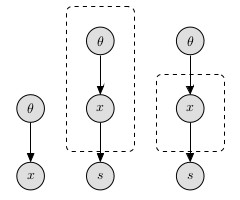
\includegraphics{plots/figure_A.jpg}
% \end{center}
% \caption{\label{fig:Plate notation, simple example} Three simple selection models. {\bf (left)} the original $p(x,\theta)$; {\bf (middle)} the model $q_{\left\{ x,\theta\right\} }$, where $\theta$ and $x$ are
% sampled together until $s=1$; {\bf (right)} the model $q_{x}$, where only $x$ is sampled until $s=1$.}
% \end{figure}

% Let $f(x,\theta\mid\eta)=f(x\mid\theta,\eta)p(\theta)$ be the joint density of a random effects meta-analysis, where $x$ is the effect size, $\theta$ is the study-specific parameter of interest, and $\eta$ is a study-specific nuisance parameter such as the sample size of the study. The left plot of Figure \ref{fig:Plate notation, simple example} is a visualization of $f(x,\theta)$. If we have more than one study to analyse, we will have to work with product density $\prod_{i=1}^{n}f(x_{i},\theta_{i}\mid\eta_{i})$ instead of the stand-alone density $f(x,\theta\mid\eta)$. This is visualised in the middle plot of Figure \ref{fig:Plate notation, simple example}  by drawing a solid plate around the pair $(x,\theta)$. When we are dealing with a fixed effects meta-analysis, in which $\theta$ is fixed, the plate should be drawn around $x$ only (Figure \ref{fig:Plate notation, simple example}, right graph). 

% \subsubsection*{Graphical representation of the publication bias and $p$-hacking models}

% To visualize selection models based on \textit{p}-values, we must make some modifications to the original graph: (i) Add the \textit{p}-value node $u$; (ii) Add an arrow from $x$ to $u$; (iii) Since the \textit{p}-value $u$ usually depends on more information than just $x$, such as the standard deviation of $x$, add an arrow from $\eta$ (which represents the extra information) to $u$ as well; (iv) Add the selection node $s$ and an arrow from $u$ to $s$. If $u$ is the only parent of $s$, we are dealing with selection models only based on \textit{p}-values.

% The placement of dashed and solid plates depends on which model we want to use. The idea behind the publication bias model is that a completely new study is done whenever the last one failed to be published. This implies that $\theta$ and $x$ are sampled together. The left plot of Figure \ref{fig:Plate notation, publication bias and p-hacking} shows the direct acyclic graph of the normal publication bias model defined in Proposition 3 in the main text. In this particular case, $\eta$ corresponds to $\sigma$, the standard deviation. Moreover, $u$ is a \textit{p}-value, $\theta_{0}$ is the mean of the effect size distribution, $\tau$ is the standard deviation of the effect size distribution, and $\rho$ is the selection probability function. The variable $Z$ lives on the unit interval, and encodes the editor's decision to publish: If the observed \textit{p}-value is less than $Z$, the study is published. Importantly, $Z$ is placed inside the selection set because a new \textit{p}-value cut-off decision is made for each study received. Since $x$ and $\theta$ are sampled together, the selection mechanism modifies $p(\theta)$.%, as can be seen in the example \ref{exa:Publication bias, theta distribution} here below.

% In the \textit{p}-hacking scenario, the \textit{p}-hacker will hack his study all the way to significance, regardless of $\theta$. This means that $\theta$ and $x$ are sampled separately and $\theta$ must be placed outside the selection set. Moreover, the decision of how much to \textit{p}-hack is not reevaluated at each attempt. Consequently, the random variable that controls the \textit{p}-hacking decisions, analogously to the publication bias model, $Z$, is also placed outside the selection graph. This is the case, for example, of an author who decides to \textit{p}-hack to level $\alpha$ ($Z = \alpha$): he acts on $x$ to obtain the desired \textit{p}-value, whatever the sampled $\theta$ is. The graphical representation of this model is shown in the right plot of Figure \ref{fig:Plate notation, publication bias and p-hacking}. Since $x$ and $\theta$ are not sampled together, the selection mechanism does not modify $p(\theta)$.

% \begin{figure}
% \begin{center}
% 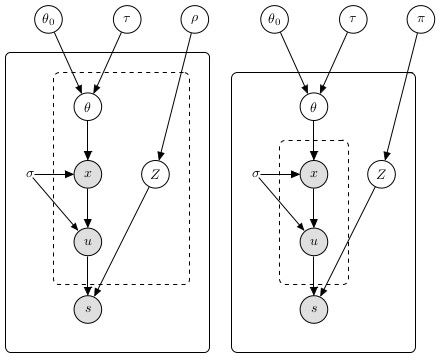
\includegraphics{plots/figure_B.jpg}
% \end{center}
% \caption{\label{fig:Plate notation, publication bias and p-hacking} Directed acyclic graphs for: {\bf (left)}
% the publication bias model; {\bf (right)} the \textit{p}-hacking model. The dashed plates enclose the selection sets and the the solid plates enclose variables that are repeated together.}
% \end{figure}


\bibliographystyle{biom}
\bibliography{main.bib}

\end{document}